% default header style
\pagestyle{fancy}
\fancyhf{}
\fancyhead[LE,RO]{\scshape\thepage}
\fancyhead[RE,LO]{
\scshape\ifnum\value{chapter}>0 \fi\leftmark}
\renewcommand{\headrulewidth}{.5pt}
\setlength{\headheight}{15pt}

% overridden style for chapter pages
\fancypagestyle{plain}{
\fancyhf{} 
\fancyhead[LE,RO]{\scshape\thepage}}

% overridden style for empty pages
\fancypagestyle{empty}{
\fancyhf{} 
\fancyhead[LE,RO]{\scshape\thepage}}

% additional setup
\hypersetup{pdfdisplaydoctitle = true, colorlinks = false}
\captionsetup{width=.75\textwidth}

\definecolor{shadecolor}{gray}{.95}
\graphicspath{ {./Graphics/} }

\numberwithin{equation}{chapter}

\setlength\parindent{0pt}
\allowdisplaybreaks

\tikzset{cross/.style={cross out, draw=black, minimum size=2*(#1-\pgflinewidth), inner sep=0pt, outer sep=0pt},
%default radius will be 1pt. 
cross/.default={1pt}}

\DeclareFieldFormat{titlecase}{#1}

%\makeatletter
%\renewcommand{\operator@font}{\mathgroup\symletters}
%\makeatother

\setmainfont{MinionPro}

%\def\thickhrulefill{\leavevmode \leaders \hrule height 1ex \hfill \kern \z@}
%\def\@makechapterhead#1{%
%  {\parindent \z@ \centering \reset@font
%        \thickhrulefill\quad
%        \scshape {\Large{\@chapapp{} \thechapter}}
%        \quad \thickhrulefill
%        \par\nobreak
%        \vspace*{10\p@}%
%        \interlinepenalty\@M
%        \hrule
%        \vspace*{10\p@}%
%        \Huge \bfseries\scshape #1\par\nobreak
%        \par
%        \vspace*{10\p@}%
%        \hrule
%    %\vskip 40\p@
%    \vskip 50\p@
%  }}
%  
%\def\@makeschapterhead#1{%
%  {\parindent \z@ \centering \reset@font
%		\thickhrulefill\quad
%        \scshape {\Large Preamble}
%        \quad \thickhrulefill
%        \par\nobreak
%        \vspace*{10\p@}%
%        \interlinepenalty\@M        
%        \hrule
%        \vspace*{10\p@}%
%        \Huge \bfseries\scshape #1\par\nobreak
%        \par
%        \vspace*{10\p@}%
%        \hrule
%    %\vskip 40\p@
%    \vskip 50\p@
%  }}

\newcommand{\chapterstarstyle}[2]{%
\begin{minipage}[t]{0.3\linewidth}  
\vspace{0pt}% do not remove
\begin{tikzpicture}
\node[
outer sep=0pt,
text width=2.5cm,
minimum height=2.5cm,
fill=black,
font=\color{white},
align=center
] (num) {
\includegraphics[width=2.5cm]{Graphics/Diagrams/abstract_diagram/abstract_diagram}};
\node[
outer sep=0pt,
inner sep=0pt,
anchor=south,
font=\color{black}\Large\normalfont
] at ([yshift=3pt]num.north) {\textls[180]{#2}};
\end{tikzpicture}
\end{minipage}%
\begin{minipage}[t]{.7\linewidth}%
    \vspace{2pt} % do not remove
    \rule{\linewidth}{2.5pt}\\\vskip -1.75\baselineskip%
    \rule{\linewidth}{.7pt}\vskip 10pt
    {\fontsize{32pt}{48pt}\begin{flushleft}\bfseries\scshape{#1}\end{flushleft}}
\end{minipage}%
}

\titlespacing*{\chapter}{0pt}{0pt}{40pt}
\titleformat%
{\chapter}[hang]%
{\bfseries}{%
\begin{minipage}[t]{0.3\linewidth}  
\vspace{0pt}% do not remove
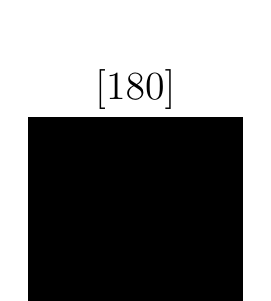
\begin{tikzpicture}
\node[
outer sep=0pt,
text width=2.5cm,
minimum height=2.5cm,
fill=black,
font=\color{white}\fontsize{80}{90}\selectfont,
align=center
] (num) {\scshape\thechapter};
\node[
outer sep=0pt,
inner sep=0pt,
anchor=south,
font=\color{black}\Large\normalfont
] at ([yshift=3pt]num.north) {\textls[180]{\textsc{\chaptertitlename}}};
\end{tikzpicture}
\end{minipage}%
}
{0pt}%
{%
\begin{minipage}[t]{.7\linewidth}%
    \vspace{2pt} % do not remove
    \rule{\linewidth}{2.5pt}\\\vskip -1.75\baselineskip%
    \rule{\linewidth}{.7pt}\vskip 10pt
    {\fontsize{32pt}{48pt}\begin{flushleft}\bfseries\scshape{#1}\end{flushleft}}
\end{minipage}%
}
  
\tikzstyle{box} = [rectangle, rounded corners, minimum width=6.5cm, minimum height=1.75cm, text centered, draw=black, fill=gray!30, thick]
\tikzstyle{header} = [rectangle, minimum width=3cm, minimum height=0.5cm, text centered, draw=black, thick, fill=white]
\tikzstyle{flowchartarrow} = [line width=0.5mm,->]

\makeatletter
\newcommand\language@yaml{yaml}

\expandafter\expandafter\expandafter\lstdefinelanguage
\expandafter{\language@yaml}
{
  keywords={True,False,null,y,n},
  keywordstyle=\color{darkgray}\mdseries\small,
  basicstyle=\YAMLkeystyle\ttfamily\mdseries\small,
  sensitive=false,
  comment=[l]{\#},
  morecomment=[s]{/*}{*/},
  commentstyle=\color{ForestGreen}\ttfamily\small,
  stringstyle=\YAMLvaluestyle\ttfamily\mdseries\small,
  moredelim=[l][\color{orange}]{\&},
  moredelim=[l][\color{magenta}]{*},
  moredelim=**[il][\YAMLcolonstyle{:}\YAMLvaluestyle]{:},
  morestring=[b]',
  morestring=[b]",
  literate =    {>}{{\textcolor{red}\textgreater}}1
                {|}{{\textcolor{red}\textbar}}1
                {\ -\ }{{\mdseries\ -\ }}3,                
  lineskip=-2pt,
}

\lstset{escapeinside={(*@}{@*)}}

% switch to key style at EOL
\lst@AddToHook{EveryLine}{\ifx\lst@language\language@yaml\YAMLkeystyle\fi}
\makeatother

\makeatletter
\renewcommand{\@makeschapterhead}[1]{%
  \vspace*{0pt}%
  \chapterstarstyle{#1}{}%
  \vspace*{40pt}%
}
\makeatother

\hypersetup{
    colorlinks=true,
    urlcolor=blue,
    citecolor=blue,
    linkcolor=blue,
    breaklinks=true
}

% If you want to break on URL numbers
\setcounter{biburlnumpenalty}{9000}
% If you want to break on URL lower case letters
\setcounter{biburllcpenalty}{9000}
% If you want to break on URL UPPER CASE letters
\setcounter{biburlucpenalty}{9000}
